\documentclass{beamer}
\usepackage{bookmark}
\usepackage{amsmath}
\usepackage{tabularx}
\usepackage{graphicx}
\usepackage{subcaption}
\usepackage{tikz}
\usetikzlibrary{arrows.meta,automata,quotes,positioning,babel}
\usetikzlibrary{shapes.geometric, arrows}
\usepackage{hyperref}
\usepackage{float}

\title{A Deep Learning Approach to Link Weight Prediction}
\author{Yuchen Hou}
\date{}

\begin{document}

\frame{
	\titlepage
	\begin{figure}[H]
		\centering
		
\includegraphics[width=0.5\linewidth]{WSU}
		\label{fig:WSU}
	\end{figure}
}

\begin{frame}{Introduction: deep learning in different application domains}
%	\begin{itemize}[<+->]
	\begin{itemize}
		\item Image recognition
		\item Speech recognition
		\item Natural language processing
		\item Graph mining
	\end{itemize}
\end{frame}

\begin{frame}{Background: graph mining problems}
	\begin{figure}[H]
		\centering
		\begin{subfigure}{0.49\textwidth}
			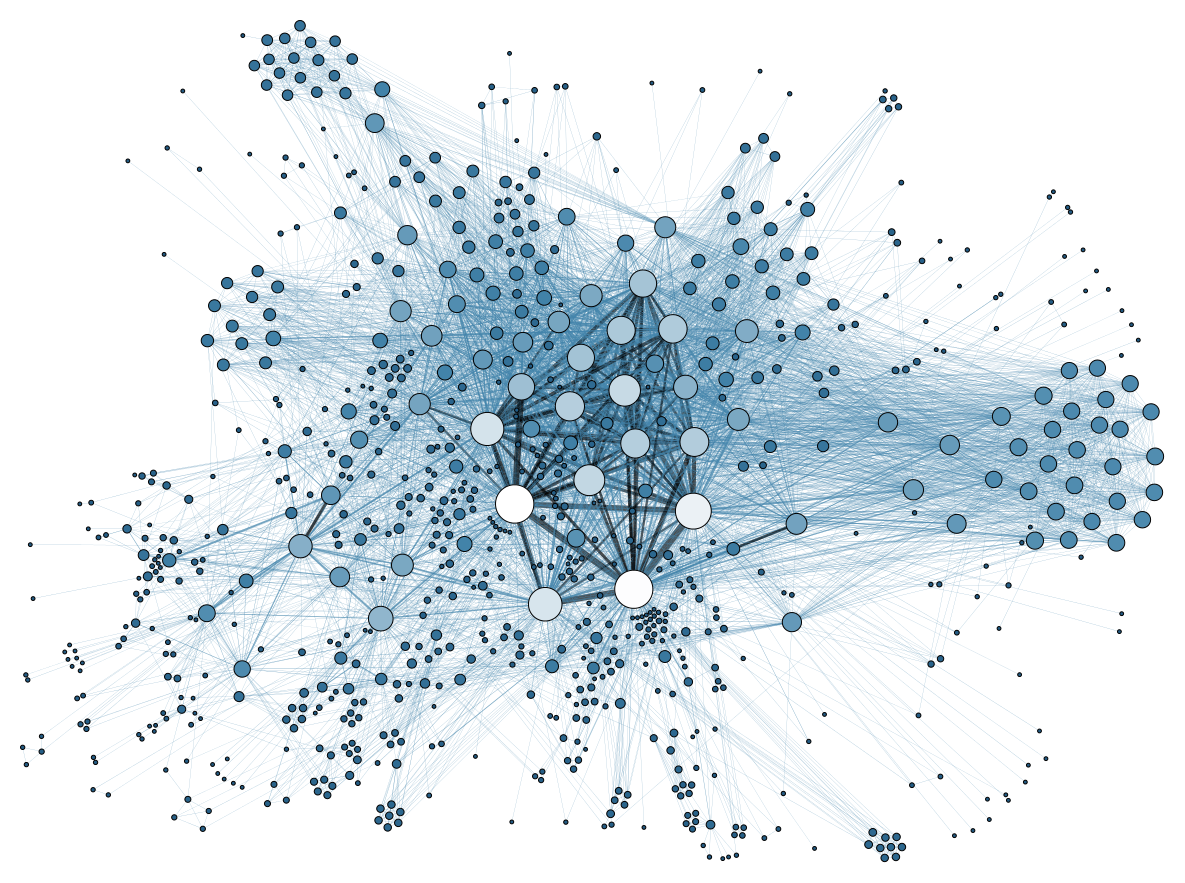
\includegraphics[width=\linewidth]{Social_Network_Analysis_Visualization}
			\caption{
				Link prediction: predicting user connectivities in a social network.
			}
			\label{fig:Social_Network_Analysis_Visualization}
		\end{subfigure}
		\begin{subfigure}{0.49\textwidth}
			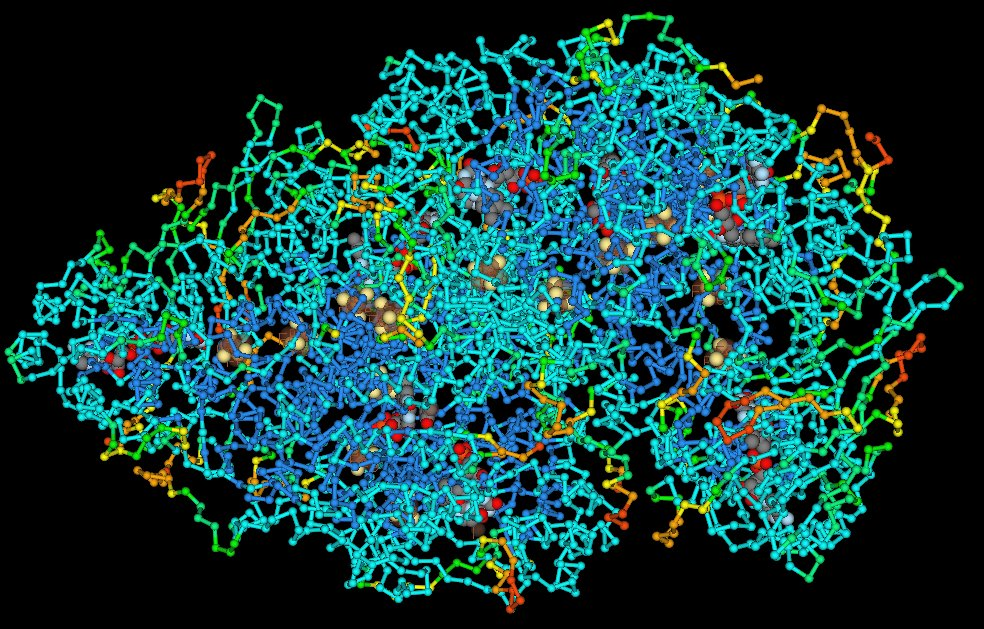
\includegraphics[width=\textwidth]{ProteinStructure}
			\caption{
				Graph classification: predicting the chemical activity of a macromolecule.
			}
			\label{fig:protein}
		\end{subfigure}
		\caption{
			Example graph mining problems and their application scenarios.
		}
		\label{fig:trainnig}
	\end{figure}
\end{frame}

\begin{frame}{Contribution: link weight prediction with deep learning}
	\begin{itemize}
		\item The first deep learning approach to the link weight prediction problem.
		\item A unique supervised learning technique for node embedding.
		\item 73\% more accurate than the state-of-the-art non deep learning approach.
		\item A generalized link weight prediction model using pretrained node embeddings.
	\end{itemize}
\end{frame}

\begin{frame}{Problem: link weight prediction}{Problem example}
	\begin{figure}[H]\centering
		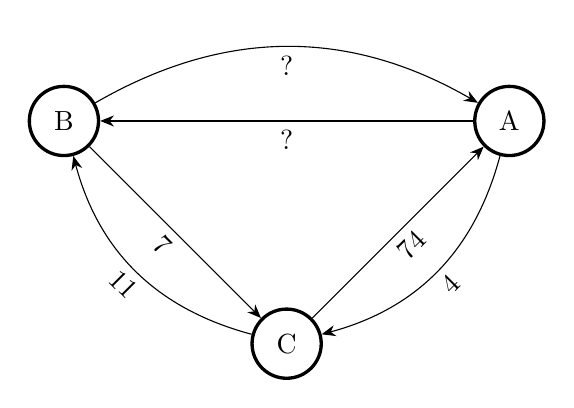
\begin{tikzpicture}[
		node distance = 4cm,
		on grid,
		> = {Stealth[length=5pt,width=4pt]},
		every state/.style = {very thick},
		every edge quotes/.style = {sloped, anchor=north}
		]
		\node[state] (B) {B};
		\node[state] (C) [below right=of B] {C};
		\node[state] (A) [above right=of C] {A};
		\path[->]   
		(A) edge["?"]   (B)
		(B) edge["7"]   (C)
		(C) edge["74"]  (A)
		(B) edge[bend left,"?"]   (A)
		(A) edge[bend left,"4"]   (C)
		(C) edge[bend left,"11"]  (B);
		\end{tikzpicture}
		\caption{Message volume prediction in a social network of 3 users.}
		\label{fig:example}
	\end{figure}
\end{frame}

\begin{frame}{Problem: link weight prediction}{Problem definition}
	\begin{itemize}
		\item Given a weighted directed graph with the node set V and a link subset E
		\item Build a model weight = f(source, destination) to predict the weight of any link (source, destination) $ \notin $ E
	\end{itemize}
\end{frame}

\begin{frame}{The state-of-the-art approach} {pWSBM (pure Weighted Stochastic Block Model)}
	\begin{itemize}
		\item Partition nodes into node groups of topologically similar nodes.
		\item Connect groups with bundles with normal weight distributions.
		\item A bundle represents all links connecting the two groups.
		\item A link has the same weight distribution as the bundle representing it.
	\end{itemize}
	\begin{figure}[H]
		\centering
		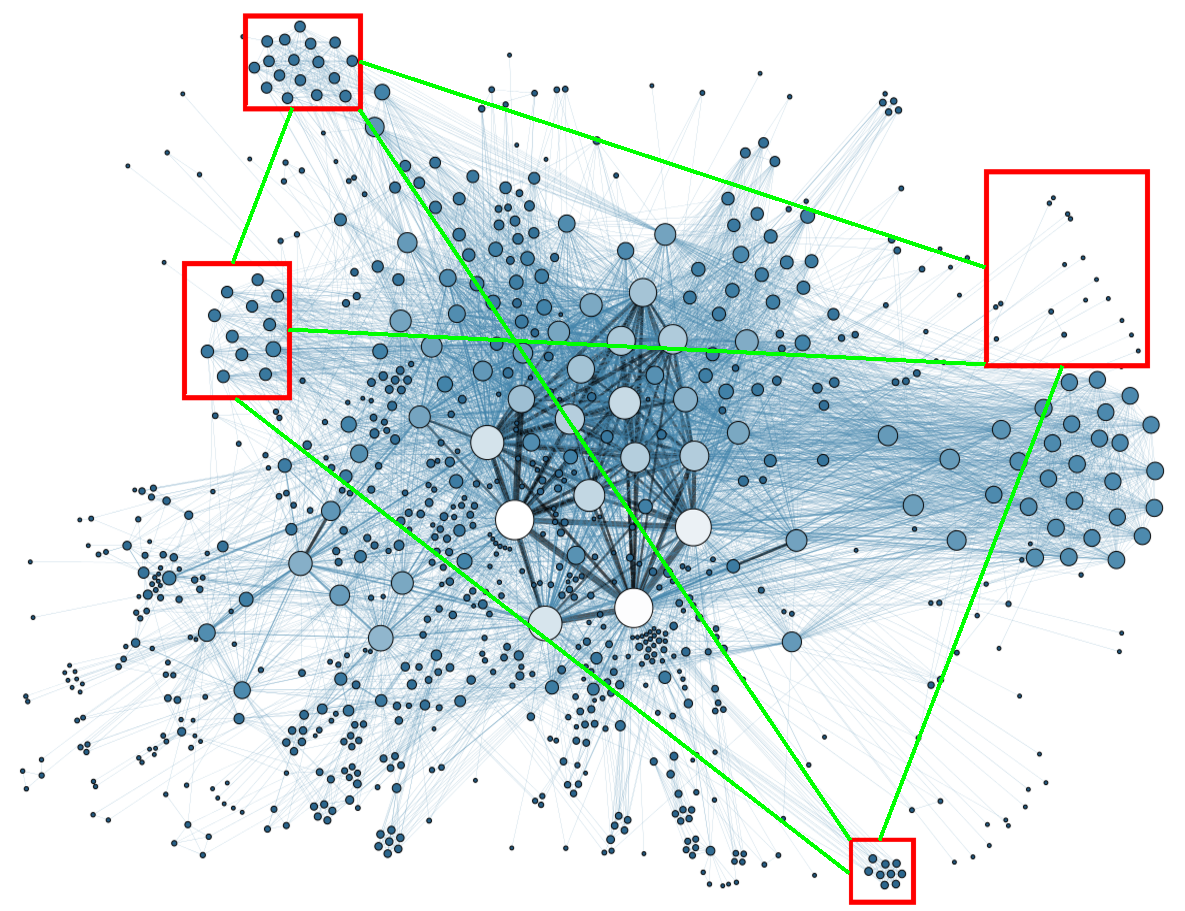
\includegraphics[width=0.4\linewidth]{SBM}
		\caption{ \href{https://commons.wikimedia.org/wiki/File:Social_Network_Analysis_Visualization.png}{pWSBM approach to link weight prediction.}}
		\label{fig:SBM}
	\end{figure}
\end{frame}

\begin{frame}{The state-of-the-art approach} {pWSBM (pure Weighted Stochastic Block Model)}
	The SBM has the following parameters:
	\begin{itemize}
		\item z: the node group label vector
		\item $ \mu $: the bundle weight expectation matrix
		\item $ \sigma $: the bundle weight standard deviation matrix
	\end{itemize}
	The weight of each link (i, j) $ A_{ij} $ has normal distribution:
	\begin{align*}
		A_{ij} \sim N(\mu_{z_i z_j}, \sigma_{z_i z_j}^2)
	\end{align*}
	The pWSBM fits parameter z, $ \mu $ and $ \sigma $
	to maximize the log likelihood of observation A:
	\begin{align*}
		\log(P(A|z, \mu, \sigma))
		&= \sum_{ij} (
		\frac{\mu_{z_i z_j}}{\sigma_{z_i z_j}^2}
		- \frac{1}{2\sigma_{z_i z_j}^2}
		- \frac{\mu_{z_i z_j}^2}{\sigma_{z_i z_j}^2}
		)
	\end{align*}
\end{frame}

\begin{frame}{Motivation: Skip-gram model}{Model architecture}
	\begin{itemize}
		\item word2vec: map words in sentences to vectors.
		\item item2vec: reduce orders (lists of items) to sentences.
		\item node2vec: reduce paths (lists of nodes) to sentences.
	\end{itemize}
	\begin{figure}[H]
		\centering
		\newcommand{\layersep}{2cm}
		\newcommand{\vocabularySize}{4}
		\newcommand{\embeddingSize}{2}
		\begin{tikzpicture}[shorten >=1pt,->,draw=black!50, node distance=\layersep]
		\tikzstyle{every pin edge}=[<-,shorten <=1pt]
		\tikzstyle{neuron}=[circle,fill=black!25,minimum size=16pt,inner sep=0pt]
		\tikzstyle{input neuron}=[neuron, fill=green!50];
		\tikzstyle{output neuron}=[neuron, fill=red!50];
		\tikzstyle{hidden neuron}=[neuron, fill=blue!50];
		\tikzstyle{annot} = [text width=4em, text centered]
		
		% Draw the input layer
		\foreach \name / \y in {1,...,\vocabularySize}
		% This is the same as writing \foreach \name / \y in {1/1,2/2,3/3,4/4}
		\node[input neuron, pin=left:$ w_\y $] (I-\name) at (0,-\y) {};
		
		% Draw the hidden layer
		\foreach \name / \y in {1,...,\embeddingSize}
		\path[yshift=-1cm]
		node[hidden neuron] (H-\name) at (\layersep,-\y cm) {};
		
		% Draw the output layer
		\foreach \name / \y in {1,...,\vocabularySize}
		\node[output neuron, pin={[pin edge={->}]right:$ w_\y $}] (O-\name) at (2*\layersep,-\y) {};
		
		% Connect the input layer with the hidden layer
		\foreach \source in {1,...,\vocabularySize}
		\foreach \dest in {1,...,\embeddingSize}
		\path (I-\source) edge (H-\dest);
		
		% Connect the hidden layer with the output layer
		\foreach \source in {1,...,\embeddingSize}
		\foreach \dest in {1,...,\vocabularySize}
		\path (H-\source) edge (O-\dest);
		
		% Annotate the layers
		\node[annot,above of=H-2] {embedding layer};
		\node[annot,above of=I-2] {input layer};
		\node[annot,above of=O-2] {output layer};
		\end{tikzpicture}	
		\caption{The skip-gram model with vocabulary size 4 and embedding size 2.}
		\label{fig:skipGram}
	\end{figure}
\end{frame}

\begin{frame}{Motivation: Skip-gram model}{Datasets}
	\begin{itemize}
		\item Sentence: the quick brown fox jumps over the lazy dog
		\item Context radius: 2
		\item Training example: (word, context-word) pairs
	\end{itemize}
	\begin{table}[H]\centering
		\caption{The words dataset for a natural language corpus.}
		\begin{tabular}{|c|c|}  \hline
			\textbf{Input = word} & \textbf{Output = context-word} \\ \hline
			fox & quick \\ \hline
			fox & brown \\ \hline
			fox & jumps \\ \hline
			fox & over \\ \hline
			jumps & brown \\ \hline
			jumps & fox \\ \hline
			... & ...       \\ \hline
		\end{tabular}
		\label{tab:words}
	\end{table}
\end{frame}

\begin{frame}{Deep learning approach: Model R (R as in "relation")}
	\begin{figure}[H]
		\centering
		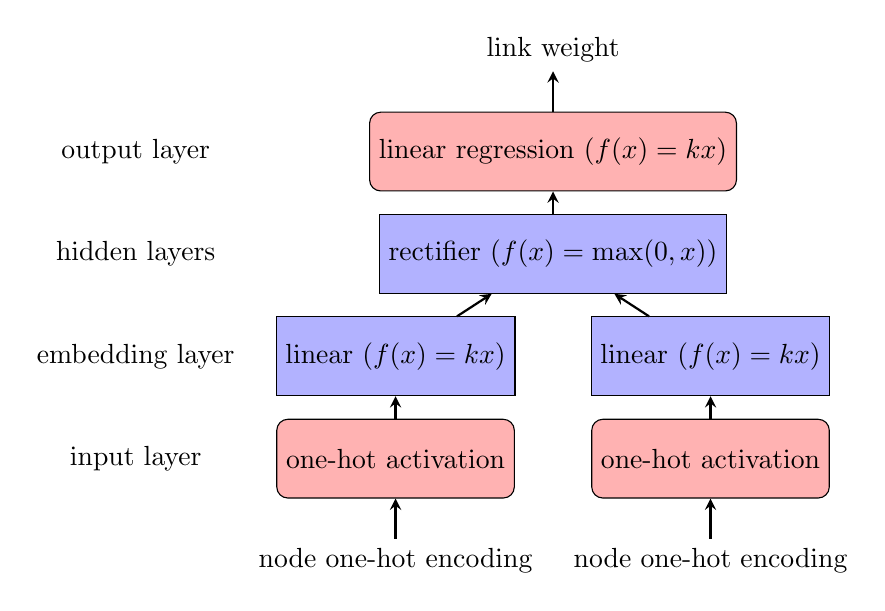
\begin{tikzpicture}[node distance=1.3cm]
		\tikzstyle{startstop} = [rectangle, rounded corners, minimum width=1cm, 
		minimum height=1cm, text centered, draw=black, fill=red!30]
		\tikzstyle{process} = [rectangle, minimum width=1cm, minimum height=1cm, 
		text centered, draw=black, fill=blue!30]
		\tikzstyle{arrow} = [thick,->,>=stealth]
		\node (linearRegression) [startstop] {linear regression ($ f(x) = kx $)};
		\node (relu) [process, below of=linearRegression] {rectifier ($ f(x) = \max (0, x) $)};
		\node (linear1) [process, below of=relu, xshift=-2cm] {linear ($ f(x) = kx $)};
		\node (linear2) [process, below of=relu, xshift=2cm] {linear ($ f(x) = kx $)};
		\node (oneHot1) [startstop, below of=linear1] {one-hot activation};
		\node (oneHot2) [startstop, below of=linear2] {one-hot activation};
		\node (weight) [above of=linearRegression] {link weight};
		\node (output) [left of=linearRegression, xshift=-4cm] {output layer};
		\node (hidden) [below of=output] {hidden layers};
		\node (embedding) [below of=hidden] {embedding layer};
		\node (input) [below of=embedding] {input layer};
		\node (source) [below of=oneHot1] {node one-hot encoding};
		\node (destination) [below of=oneHot2] {node one-hot encoding};
		\draw [arrow] (source) -- (oneHot1);
		\draw [arrow] (destination) -- (oneHot2);
		\draw [arrow] (oneHot1) -- (linear1);
		\draw [arrow] (oneHot2) -- (linear2);
		\draw [arrow] (linear1) -- (relu);
		\draw [arrow] (linear2) -- (relu);
		\draw [arrow] (relu) -- (linearRegression);
		\draw [arrow] (linearRegression) -- (weight);
		\end{tikzpicture}
		\caption{
			Model R with multiple hidden layers.
		}
		\label{fig:model}
	\end{figure}
\end{frame}

\begin{frame}{Comparison: pWSBM vs Model R}
	\begin{table}[H]\centering
		\caption{The advantages Model R has over pWSBM in several aspects.}
		\begin{tabular}{|c|c|c|}  \hline
			\textbf{Aspect} & \textbf{pWSBM} & \textbf{Model R} \\ \hline
			model granularity & node group level & node level \\ \hline
			distribution assumption & normal distribution & NA \\ \hline
			model flexibility & low & high \\ \hline
		\end{tabular}
		\label{tab:comparison}
	\end{table}
\end{frame}

\begin{frame}{Experiments}{Baseline approaches}
	\begin{itemize}
		\item SBM (Stochastic Block Model)
		\item pWSBM (pure Weighted Stochastic Block Model)
		\item bWSBM (balanced Weighted Stochastic Block Model)
		\item DCWBM (Degree Corrected Weighted Stochastic Block Model)
	\end{itemize}
\end{frame}

\begin{frame}{Experiments}{Datasets}
	\begin{table}[H]\centering
		\caption{The datasets used in experiments with weights scaled to [0, 1].}
		\begin{tabular}{|c|c|c|}  \hline
			\textbf{Dataset} & \textbf{Nodes} & \textbf{Link weights} \\ \hline
			Airport & airports & passengers delivered between airports \\ \hline
			Collaboration & nations & paper collaborations between nations \\ \hline
			Congress & committees  & members shared between committees \\ \hline
			Forum  & users & messages exchanged between users \\ \hline
		\end{tabular}
		\label{tab:datasets}
	\end{table}
\end{frame}

\begin{frame}{Experiments}{Settings}
	\begin{itemize}
		\item 25 independent trials on each dataset
		\item training set: 70\%
		\item validation set: 20\%
		\item testing set: 10\%
	\end{itemize}
\end{frame}

\begin{frame}{Experiments}{Results}
	\begin{figure}[H]\centering
		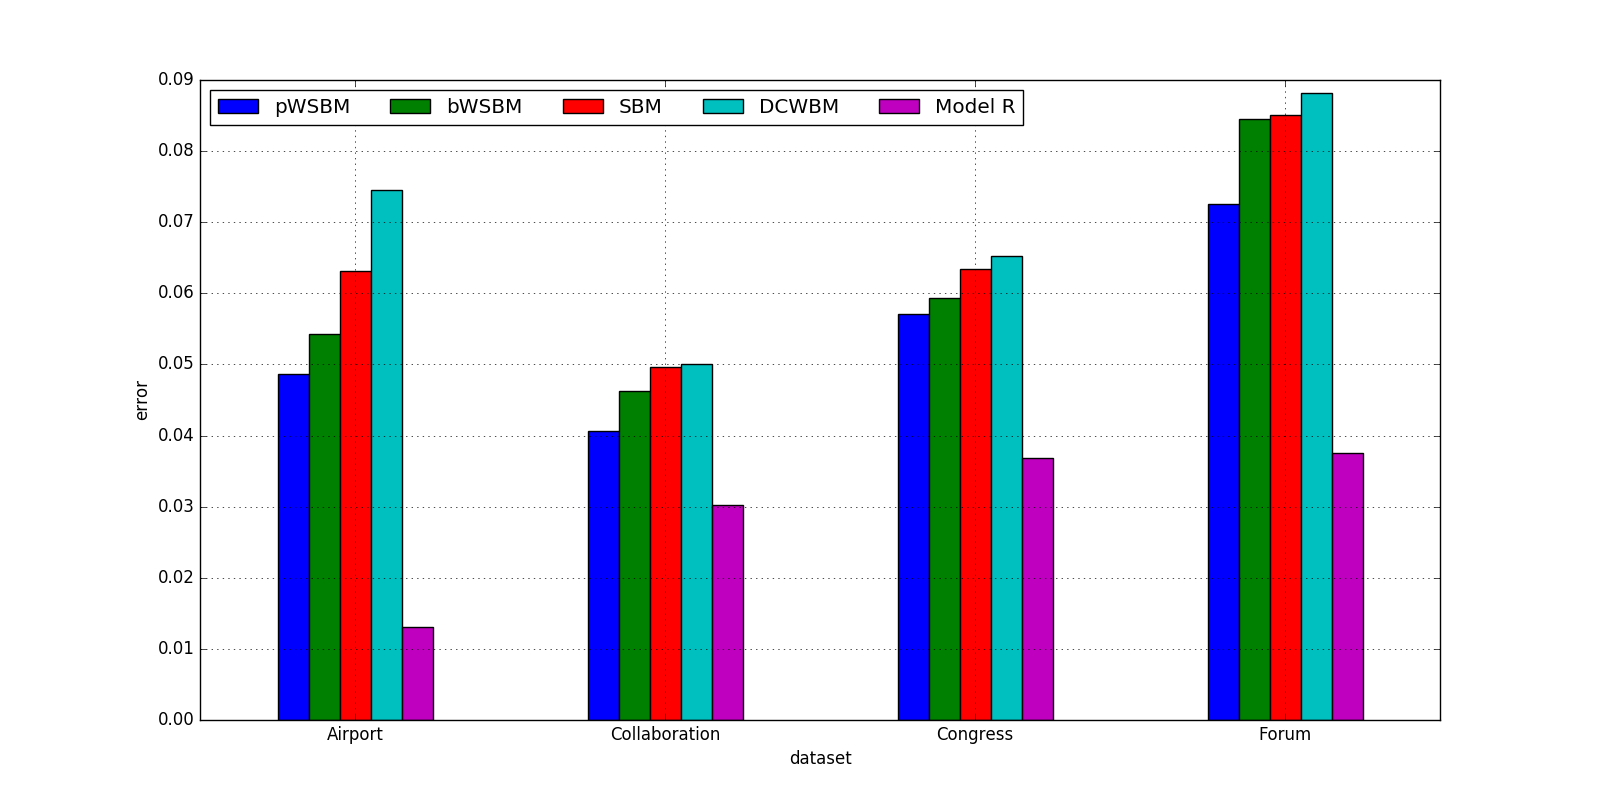
\includegraphics[width=\textwidth]{link-weight-errors}
		\caption{
			Model R has lower mean squared errors than 4 baseline approaches over 4 datasets consistently.
		}
		\label{fig:errors}
	\end{figure}
\end{frame}

\begin{frame}{Node embedding analysis}{Motivation}
	\begin{itemize}
		\item Question: What knowledge does Model R learn?
		\item Hypothesis: It learns meaningful node embeddings (similar nodes are closer).
		\item Related work: Word2vec word embedding analysis.
	\end{itemize}
\end{frame}

\begin{frame}{Node embedding analysis}{Dataset: MovieLens 100K}
	\begin{itemize}
		\item Well understood domain: movie recommendation
		\item 100,000 ratings from 1000 users on 1700 movies.
		\item Bigraph: users and movies are nodes; ratings are link weights.
	\end{itemize}
	\begin{figure}[H]\centering
		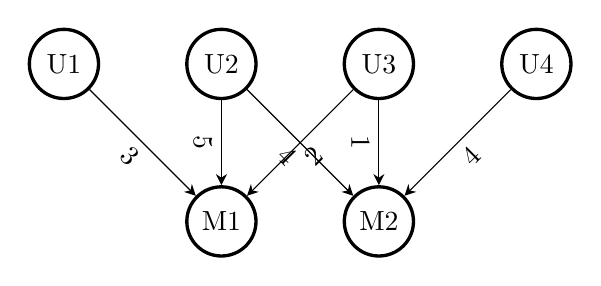
\begin{tikzpicture}[
		node distance = 2cm,
		on grid,
		> = {Stealth[length=4pt,width=4pt]},
		every state/.style = {very thick},
		every edge quotes/.style = {sloped, anchor=north}
		]
		\node[state] (U1) {U1};
		\node[state] (U2) [right =of U1] {U2};
		\node[state] (U3) [right =of U2] {U3};
		\node[state] (U4) [right =of U3] {U4};
		\node[state] (M1) [below=of U2] {M1};
		\node[state] (M2) [right =of M1] {M2};
		\path[->]
		(U1) edge["3"]   (M1)
		(U2) edge["5"]   (M1)
		(U2) edge["4"]  (M2)
		(U3) edge["2"]   (M1)
		(U3) edge["1"]   (M2)
		(U4) edge["4"]   (M2);
		\end{tikzpicture}
		\caption{Movie rating illustration for a dataset of 4 users and 2 movies.}
		\label{fig:movie}
	\end{figure}
\end{frame}

\begin{frame}{Node embedding analysis}{Visualization}
	\begin{figure}[!ht]\centering
		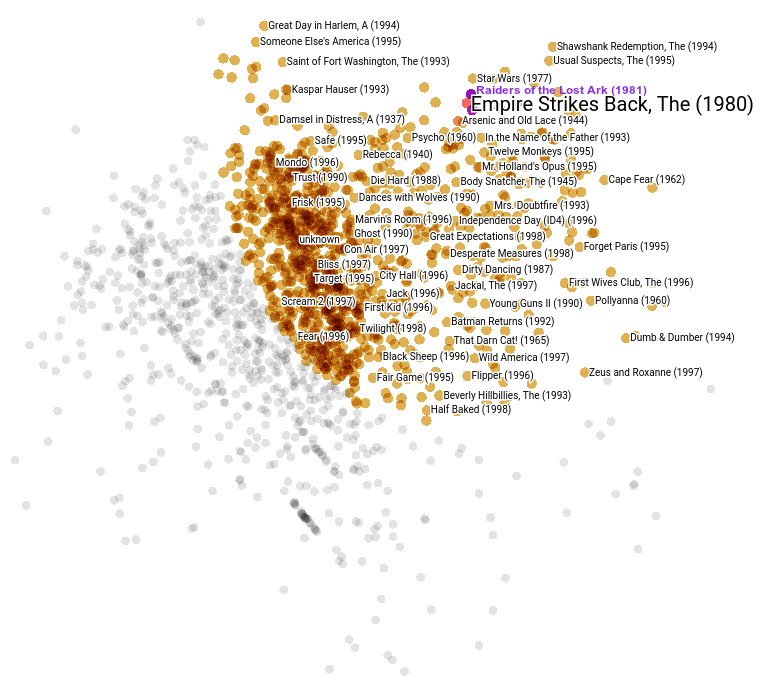
\includegraphics[width=0.6\textwidth]{movies-annotation}
		\caption{
			The embeddings of all movies in MovieLens 100K dataset. Dimensionality reduction of embeddings uses Principal Component Analysis.
		}
		\label{fig:movies}
	\end{figure}
\end{frame}

\begin{frame}{Node embedding analysis}{Distance and similarity}
	\begin{table}[H]\centering
		\caption{
			The distances of movies to the reference movie for MovieLens 100K dataset. The distance from similar movies (Star Wars and Return of Jedi) to the reference movie (The Empire Strikes Back) are shorter than the median distance.
		}
		\begin{tabular}{|c|c|c|} \hline
			\textbf{Movie} & \textbf{Distance} & \textbf{Similarity} \\ \hline
			The Empire Strikes Back (1980) & 0 & self (reference) \\ \hline
			Raiders of the Lost Ark (1981) & 0.012 & most similar \\ \hline
			Star Wars (1977) & 0.047 & more similar \\ \hline
			Return of the Jedi (1983) & 0.063 & more similar \\ \hline
			Children of the Revolution (1996) & 0.256 & median point \\ \hline
			Tomorrow Never Dies (1997) & 0.295 & less similar \\ \hline
			Ayn Rand: A Sense of Life(1997) & 0.296 & less similar \\ \hline
			101 Dalmatians (1996) & 0.335 & least similar \\ \hline
		\end{tabular}
		\label{tab:movielens100k-distance}
	\end{table}
\end{frame}

\begin{frame}{Model S}{Motivation}
	\begin{itemize}
		\item Model S is an extension of Model R incorporating different types of embeddings.
		\item Decoupling node embedding learning and weight prediction learning.
		\item Investigating the effectiveness of other node embedding techniques.
		\item Adopting more advanced embedding techniques developed in the future.
	\end{itemize}
\end{frame}

\begin{frame}{Model S}{Node embedding techniques}
	\begin{itemize}
		\item LLE(locally linear embedding): nonlinear dimensionality reduction
		\item Node2vec: node embedding with skip-gram model
		\item Model R: node embedding learning supervised by link weight
	\end{itemize}
\end{frame}

\begin{frame}{Model S}{LLE(locally linear embedding)}
	LLE is a manifold learning approach designed for dimensionality reduction consisting of 2 steps:
	\begin{enumerate}
		\item Linear approximation of data points X's in original space minimizing cost function:
		\begin{align*}
			cost(W) = \sum_i |X_i - \sum_jW_{ij}X_j|^2
		\end{align*}
		\item Reconstruction of data points Y's in a low dimensional space minimizing cost function:
		\begin{align*}
		cost(Y) = \sum_i |Y_i - \sum_jW_{ij}Y_j|^2
		\end{align*}
	\end{enumerate}
\end{frame}

\begin{frame}{Model S}{Experiments}
	\begin{figure}[ht] \centering
		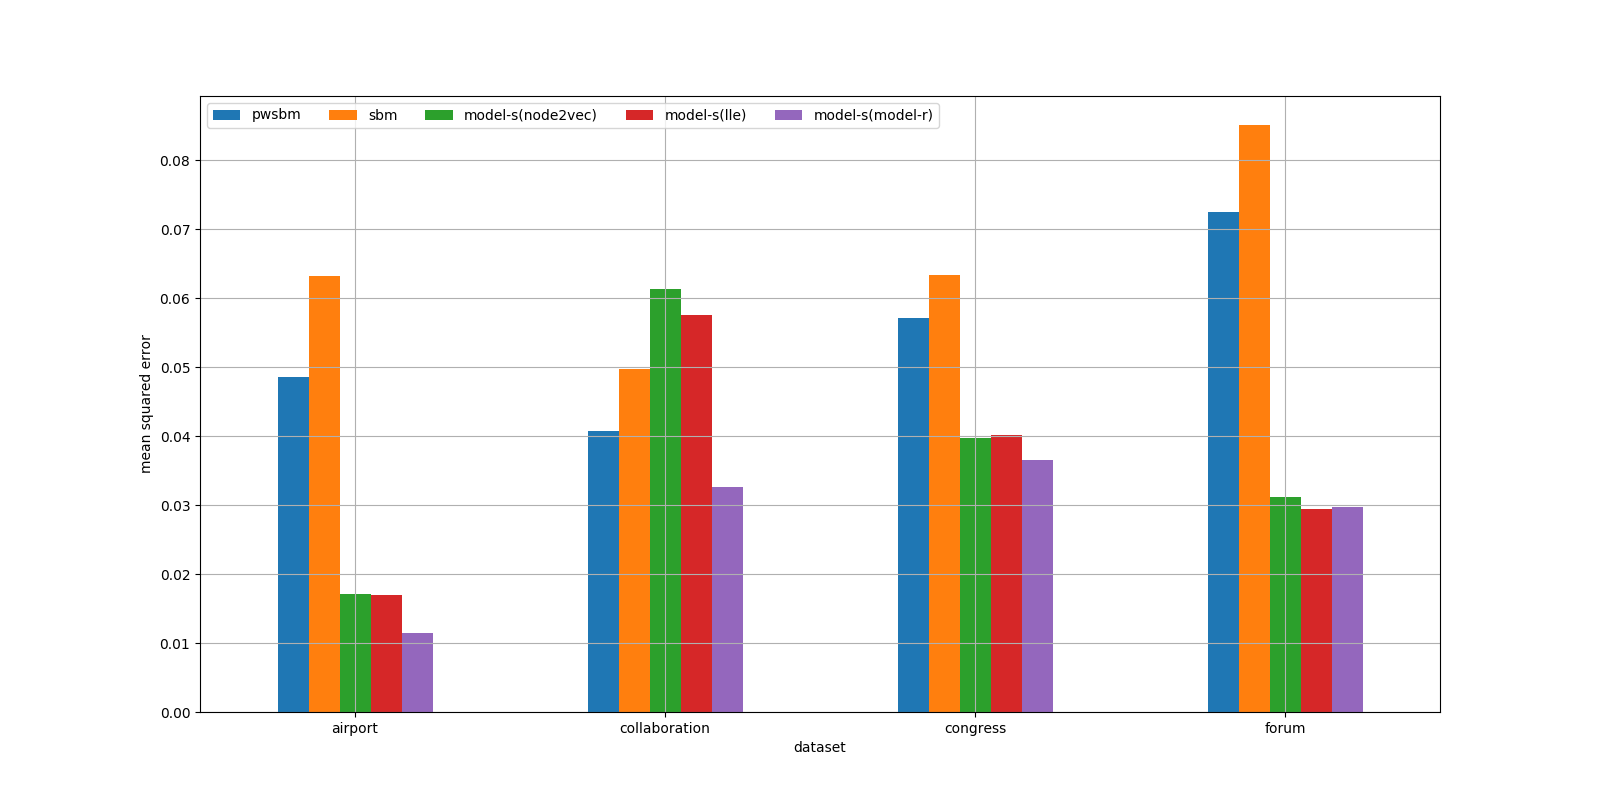
\includegraphics[width=1\linewidth]{weight-errors}
		\caption{
			Model S with Model R embedding has the best overall performance. Model S generally performs better than SBM and pWSBM with 3 different embedding techniques (LLE, Model R and node2vec).
		}
		\label{fig:weight-errors}
	\end{figure}
\end{frame}

\begin{frame}{Conclusions}
	\begin{itemize}
		\item Model R is more accurate than the state-of-the-art non deep learning approaches to the link weight prediction problem.
		\item Model R learns node embeddings and uses this information to predict unknown link weights.
		\item Deep learning can be successfully applied to link weight prediction problem.
	\end{itemize}
\end{frame}

\begin{frame}{Future work}
	\begin{itemize}
		\item Unified node embedding: embedding nodes to only one space.
		\item Node embedding metrics: evaluation of embedding qualities.
		\item Complex graphs: taking advantage of rich node information.
	\end{itemize}
\end{frame}

\begin{frame}{Publications}
	\begin{itemize}
		\item Comparative analysis of deep node embeddings for link weight prediction in graphs, TNNLS 2018 (in preparation)
		\item On graph mining with deep learning: introducing Model R for link weight prediction, JAISCR 2018
		\item Deep learning approach to link weight prediction, IJCNN 2017
	\end{itemize}
\end{frame}

\begin{frame}
	\begin{center}
		\Huge Thank you!
	\end{center}
\end{frame}
\end{document}